%%%%%%%%%%%%%%%%%%%%%%%%%%%%%%%%%%%%%%%%%%%%%%%%%%%%%%%%%%%%%%%%%%%%%%%%%%%%%
% Forked from Beamer Template by Bill Lampos
%
% Feel free to use (copy) the structure (latex formatting source code)
% but not the content of this document.
%
% Author: Primal Pappachan
% Date: 2 - 10 - 2012
% Images by : Satyajit Sarangi
%%%%%%%%%%%%%%%%%%%%%%%%%%%%%%%%%%%%%%%%%%%%%%%%%%%%%%%%%%%%%%%%%%%%%%%%%%%%%
\documentclass[compress,red]{beamer}
\mode<presentation>

\usetheme{Warsaw}
% other themes: AnnArbor, Antibes, Bergen, Berkeley, Berlin, Boadilla, boxes, CambridgeUS, Copenhagen, Darmstadt, default, Dresden, Frankfurt, Goettingen,
% Hannover, Ilmenau, JuanLesPins, Luebeck, Madrid, Maloe, Marburg, Montpellier, PaloAlto, Pittsburg, Rochester, Singapore, Szeged, classic

%\usecolortheme{lily}
% color themes: albatross, beaver, beetle, crane, default, dolphin, dov, fly, lily, orchid, rose, seagull, seahorse, sidebartab, structure, whale, wolverine

%\usefonttheme{serif}
% font themes: default, professionalfonts, serif, structurebold, structureitalicserif, structuresmallcapsserif

% pdf is displayed in full screen mode automatically
%\hypersetup{pdfpagemode=FullScreen}

% define your own colours:
\definecolor{Red}{rgb}{1,0,0}
\definecolor{Blue}{rgb}{0,0,1}
\definecolor{Green}{rgb}{0,1,0}
\definecolor{magenta}{rgb}{1,0,.6}
\definecolor{lightblue}{rgb}{0,.5,1}
\definecolor{lightpurple}{rgb}{.6,.4,1}
\definecolor{gold}{rgb}{.6,.5,0}
\definecolor{orange}{rgb}{1,0.4,0}
\definecolor{hotpink}{rgb}{1,0,0.5}
\definecolor{newcolor2}{rgb}{.5,.3,.5}
\definecolor{newcolor}{rgb}{0,.3,1}
\definecolor{newcolor3}{rgb}{1,0,.35}
\definecolor{darkgreen1}{rgb}{0, .35, 0}
\definecolor{darkgreen}{rgb}{0, .6, 0}
\definecolor{darkred}{rgb}{.75,0,0}

\xdefinecolor{olive}{cmyk}{0.64,0,0.95,0.4}
\xdefinecolor{purpleish}{cmyk}{0.75,0.75,0,0}

% \usepackage{beamerinnertheme_______}
% inner themes include circles, default, inmargin, rectangles, rounded

%\usepackage{beamerouterthemesmoothbars}
% outer themes include default, infolines, miniframes, shadow, sidebar, smoothbars, smoothtree, split, tree

\useoutertheme[subsection=false]{smoothbars}

% to have the same footer on all slides
%\setbeamertemplate{footline}[text line]{xxx xxx xxx}
%\setbeamertemplate{footline}[text line]{} % or empty footer

% include packages
\usepackage{subfigure}
\usepackage{multicol}
\usepackage{amsmath}
\usepackage{epsfig}
\usepackage{graphicx}
\usepackage{graphics}
\usepackage[all,knot]{xy}
\xyoption{arc}
\usepackage{url}
\usepackage{multimedia}
\usepackage{hyperref}
\usepackage{setspace}

\title{FOSSEE}
\subtitle{Free and Open source Software for Science and Engineering
Education}
\author{}
\institute{IIT Bombay}
\date{}

\begin{document}

\frame{
  \titlepage
}



\section{General overview of the project}
\section[Outline]{}
\frame{\tableofcontents}

\subsection{Projects}
\frame{\frametitle{Projects}	
\begin{center}
{\centering {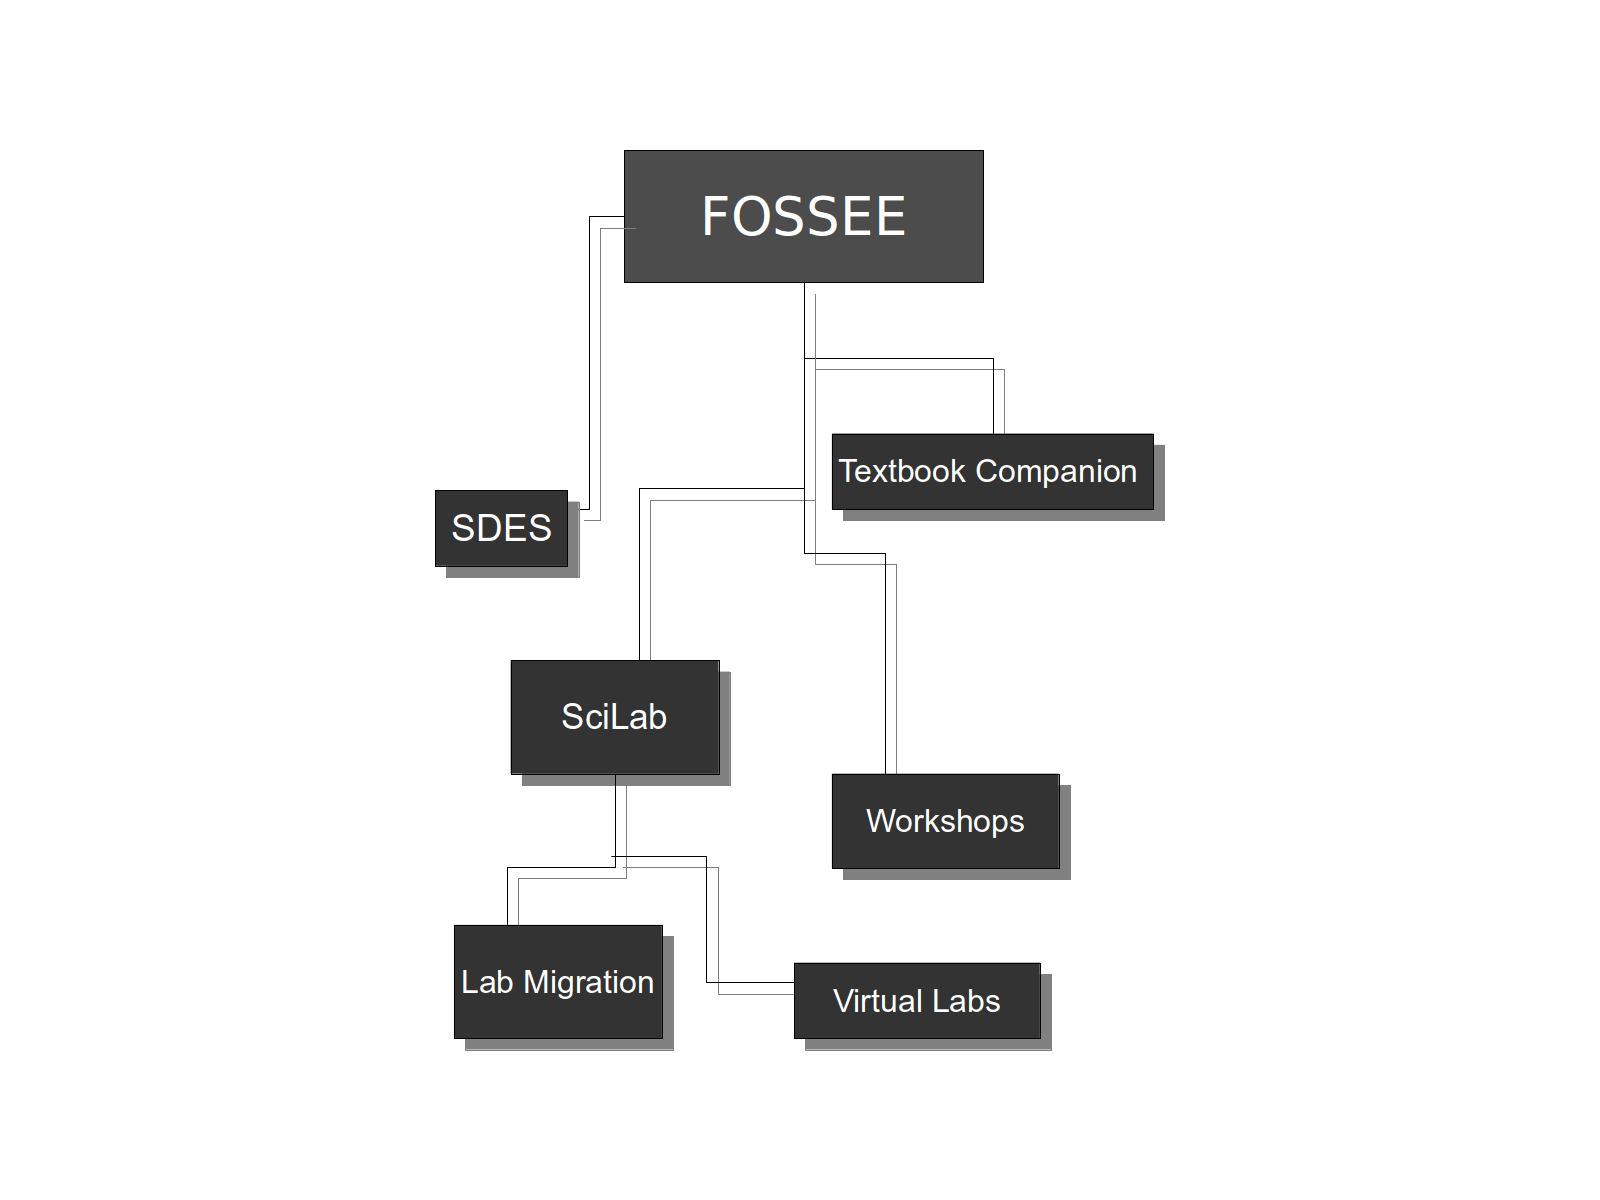
\includegraphics[scale=.14]{overview.png}}}
\end{center}
}

\section{FOSSEE}
\subsection{Introduction}
\frame{\frametitle{FOSSEE}
\begin{itemize}
\item Goals: Minimize use of commercial tools in science/engineering curriculum \pause
\item Documentation  \pause
\item Awareness. \pause
\end{itemize}
\vspace{0.25cm}
People:
\begin{itemize}
\item Prabhu Ramachandran (AE) \pause
\item Mani Bhushan (ChE) \pause
\item Madhu Belur (EE) \pause
\item Kannan Moudgalya (ChE) \pause
\end{itemize}
}

\subsection{Focus}
\frame{\frametitle{FOSSEE focus in IITB}
\begin{itemize}
\item Python family \pause
   \begin{itemize}
   \item Python
   \item NumPy
   \item SciPy
   \item Sage \pause
   \end{itemize}
\item Scilab family \pause
   \begin{itemize}
   \item Scilab
   \item Xcos \pause
   \end{itemize}
\item Other FOSS actively pursued/used \pause
   \begin{itemize}
   \item GNURadio
   \item COMEDI
   \item OpenFoam
   \item NGSpice
   \item \LaTeX % \Latex \Latex \pause
   \end{itemize}
\end{itemize}
}

\subsection{Activities}
\frame{\frametitle{Thrust Activities}
\begin{itemize}
\item SDES course \pause
\item Workshops  \pause
\item Textbook companion  \pause
\item Spoken Tutorials \pause
\end{itemize}
}

\frame{\frametitle{Development of the SDES semester-long course}
\begin{itemize}
\item Software Development Techniques for Engineers and Scientists (SDES) \pause
\item Equips a student with various FOSS tools for curricular purposes. \pause
\item For students of BE/BTech and ME/MTech programmes(Non CS/IT Streams) \pause
\item Currently in curriculum : IIT Bombay, Varanasi and Chennai \pause
\item \emph{1000 Teachers} Training for SDES through AVIEW in November 2011 \pause
\end{itemize}
}

\frame{\frametitle{Co-ordinator's workshop}
\begin{itemize}
\item Introduce the advantages of FOSS to faculty of various engineering colleges \pause
\item Motivate them to include SDES course in their curriculum. \pause
\item Conducted in 2 parts \pause
\begin{enumerate}
\item Expert faculty from remote centers to a Coordinators training workshop \pause
in IIT.
\item At selected remote centers, lecture and live transmission takes place \pause
through distance mode using AVIEW technology. \pause
\end{enumerate}
\end{itemize}
}

\frame{\frametitle{Spoken Tutorials}
\begin{itemize}
\item Create video tutorials on various modules of Python \pause
\item Can be used for self learning and teaching purposes \pause
\item To create video tutorials on various modules of Python \pause
\item Completed 37 tutorials of scientific computing using python. \pause
\item Videos can be downloaded from {\url{http://fossee.in/stvideos}} \pause
\end{itemize}
}


\section{Scilab}

\subsection{Why Scilab?}
\frame{\frametitle{Why Scilab?}
\begin{itemize}
\item Free and open source, user friendly numerical and computational package.\pause
\item Benefits of shifting to Scilab.\pause
\item Immense Capabities. \pause
\end{itemize}
}

\frame{\frametitle{What users can do?}
\begin{itemize}
\item See and modify the source code.\pause
\item Redistribute and improve the source code.\pause
\item Use the software for any purpose.\pause
\end{itemize}
This is an obvious advantage for Private Industries, Entrepreneurs, Defence Establishments, Research Organisations, Academic Institutions and Individual User. \pause
}

\subsection{Activities}
\frame{\frametitle{Activities - 1}
Some of the activities for promoting Scilab through NMEICT projects at IIT Bombay are \pause
\begin{itemize}
\item Lab Migration ( Shifting all computational laboratories to Scilab).\pause
\item Virtual Labs ( Remote Access to the Single Board Heater System:\\{\color{magenta}http://www.co-learn.in/web-sbhs}
\end{itemize}
}


\frame{\frametitle{Activities - 2}
\begin{itemize}
\item We have several spoken tutorial on Scilab at this time. \pause
\item Scilab Effort in India is co-ordinated through this website.{\color{magenta}http://scilab.in} \pause
\item There are some interesting projects one of them is the Textbook Companion project, that codes worked out examples of standard textbooks using Scilab. \pause
\item The link project allows users to link known Scilab documents and to rank them. \pause
\item We also help organize Scilab Workshops. \pause
\item We have two mailing lists one for announce and another one for discuss.\pause
\item We invite your participation in all our activities. \pause
\end{itemize}
}


\section{Statistics}
\subsection{Workshops}
\frame{\frametitle{Workshops}
{\bf \large Workshops : by FOSSEE-IITB}
\begin{itemize}
\item More than 40 workshops all over India : 30-50~participants \pause
\item Locations:\\ \pause
Durgapur, Haldia, Guwahati,  Suratkal, Hyderabad, \\
Roorkee, Kanpur, Jaipur, Delhi, Pune, Nashik \\
Cochin, Calicut, Kottayam, Bangalore, Manipal,
Chennai, Erode, Coimbatore, Surat\\
Nagpur, Mumbai, Latur, Nanded, Ramtek (near Nagpur), 
\item Spoken tutorial based 
\item Primarily \alert{targetting teachers} : 1 to 5 days \pause
\item Online test portal for quick evaluation: clearing the
online test \alert{compulsory} for participation certificate \pause
\end{itemize}
(Note: We are not counting the 2-hour-workshops.)
}

\subsection{Achievements}
\frame{\frametitle{Achievements}
\small \bf
{\bf so far (August 2011), till March 2012, till July 2012}
% {\bf Deliverables} % please give milestones with timelines linking with payments
\begin{center}
\begin{table}[h]
\begin{tabular}{|l|c|c|c|}
\hline 
Item & Aug '11 & Mar '12 & Jul '12 \tabularnewline
& (achieved) & (expected) & (proposed) \tabularnewline
\hline
\hline 
Workshops\footnote{\bf These are 1 to 5 days workshop targetted towards
\alert{teachers}, and \alert{evaluated online} before issuing a participation
certificate}  & 40 &  55 & 70\tabularnewline
\hline 
Conferences & 5 & 6 & 7 \tabularnewline
\hline 
Textbook Companions & 51 & 100 & 200 \tabularnewline
\hline 
Spoken Tutorials & 45 & 60 & 70 \tabularnewline
\hline 
Course conversion & 5 & 5 & 5\tabularnewline
\hline
Lab Migration & 4 & 10 & 20 \tabularnewline
\hline
\end{tabular}
\end{table}
\end{center}

}


\section*{}
\frame{
    \begin{center}
        \huge
        Thank you\\ \pause
    \end{center}
}

\end{document} 